\documentclass{article}
\usepackage{amsmath}
\usepackage{amssymb}
\usepackage{graphicx}
\usepackage{caption}
\usepackage[margin = 1in]{geometry}

\title{\textbf{Support Vector Machines (SVM) Applied to MNIST Dataset}}
\date{}

\begin{document}
\author{}
\date{}
\maketitle

\section*{1. Introduction}

Support Vector Machines (SVM) are a class of supervised learning algorithms designed for classification and regression tasks. Introduced by Vladimir Vapnik in the 1990s, SVM has become one of the most robust and widely used machine learning models due to its effectiveness in high-dimensional spaces and its ability to handle linear and nonlinear decision boundaries. SVM constructs a hyperplane or set of hyperplanes in a high-dimensional space to classify data points. The goal is to find the hyperplane that best separates data points of different classes while maximizing the margin, the distance between the hyperplane and the closest data points (called support vectors).

\noindent
SVM is primarily designed for:
\begin{itemize}
    \item \textbf{Binary Classification:} Separating data points into two classes by finding the optimal hyperplane.
    \item \textbf{Multiclass Classification:} Using strategies such as one-vs-one or one-vs-rest to handle more than two classes.
    \item \textbf{Regression Tasks:} Through a variation known as Support Vector Regression (SVR).
\end{itemize}

\section*{2. Mathematical formulation}

\subsection*{Linear SVM}

For a linearly separable dataset, SVM finds a hyperplane
\[
\mathbf{w} \cdot \mathbf{x} + b = 0
\]
that separates the two classes \( y_i \in \{-1, 1\} \). The objective is to maximize the margin:
\[
\text{Margin} = \frac{2}{\|\mathbf{w}\|}.
\]

\noindent
This is equivalent to solving the following optimization problem:
\[
\min_{\mathbf{w}, b} \frac{1}{2} \|\mathbf{w}\|^2
\]
subject to the constraints:
\[
y_i (\mathbf{w} \cdot \mathbf{x}_i + b) \geq 1, \quad \forall i.
\]

\subsection*{Nonlinearly Separable Data}

For data that are not linearly separable, SVM introduces slack variables \( \xi_i \) to allow misclassifications. The optimization problem becomes:
\[
\min_{\mathbf{w}, b, \xi} \frac{1}{2} \|\mathbf{w}\|^2 + C \sum_{i=1}^{n} \xi_i
\]
subject to:
\[
y_i (\mathbf{w} \cdot \mathbf{x}_i + b) \geq 1 - \xi_i, \quad \xi_i \geq 0, \quad \forall i.
\]
Here, \( C \) is a regularization parameter that controls the trade-off between maximizing the margin and minimizing the misclassification penalty.

\subsection*{Kernel Trick}
The kernel trick allows SVM to efficiently operate in high-dimensional spaces without directly computing the transformation, making it highly effective for complex, non-linear decision boundaries.
When the data is not linearly separable in its original feature space, Support Vector Machines (SVM) employ the \textit{kernel trick} to transform the data into a higher-dimensional space where linear separation may be possible. This is achieved using a feature map $\phi(\mathbf{x})$ that maps the original features into a higher-dimensional space.

\noindent
Instead of explicitly computing the feature map $\phi(\mathbf{x})$, SVM uses a kernel function $K(\mathbf{x}_i, \mathbf{x}_j)$ that computes the inner product in the transformed space:
\[
K(\mathbf{x}_i, \mathbf{x}_j) = \phi(\mathbf{x}_i)^\top \phi(\mathbf{x}_j).
\]

\noindent
Using this kernel function, the dual formulation of SVM can be expressed entirely in terms of $K(\mathbf{x}_i, \mathbf{x}_j)$, avoiding the explicit computation of $\phi(\mathbf{x})$. This enables SVM to handle very high-dimensional or even infinite-dimensional feature spaces efficiently.


\noindent
Commonly used kernel functions include:
\begin{itemize}
    \item \textbf{Linear Kernel}:
    \[
    K(\mathbf{x}_i, \mathbf{x}_j) = \mathbf{x}_i^\top \mathbf{x}_j.
    \]
    \item \textbf{Polynomial Kernel}:
    \[
    K(\mathbf{x}_i, \mathbf{x}_j) = (\mathbf{x}_i^\top \mathbf{x}_j + c)^d,
    \]
    where $c \geq 0$ and $d$ is the degree of the polynomial.
    \item \textbf{Radial Basis Function (RBF) Kernel}:
    \[
    K(\mathbf{x}_i, \mathbf{x}_j) = \exp\left(-\frac{\|\mathbf{x}_i - \mathbf{x}_j\|^2}{2\sigma^2}\right),
    \]
    where $\sigma > 0$ controls the width of the Gaussian kernel.
    \item \textbf{Sigmoid Kernel}:
    \[
    K(\mathbf{x}_i, \mathbf{x}_j) = \tanh(\alpha \mathbf{x}_i^\top \mathbf{x}_j + c),
    \]
    where $\alpha > 0$ and $c$ are kernel parameters.
\end{itemize}

\section*{3. SVM and MNIST dataset}
The MNIST dataset, comprising grayscale images of handwritten digits, is a standard benchmark for classification algorithms. Given its high-dimensional input space ($28x28$ pixels) and non-linear class boundaries, SVM is a compelling choice for this task due to its margin-maximizing property and kernel flexibility. 

\noindent
In this section we performe the implementation of SVM for the classification of the MNIST dataset. Utilizing the \texttt{scikit-learn} library, we preprocess data, train an SVM classifier, and evaluate its performance using key metrics such as accuracy and a confusion matrix. The implementation highlights the flexibility of SVM in handling high-dimensional data and non-linear class boundaries, making it suitable for tasks like handwritten digit recognition.


\subsection*{Why SVM is Suitable for MNIST Classification}

\begin{itemize}
    \item \textbf{Accuracy:} SVM provides state-of-the-art performance for many classification problems, including MNIST, especially with a well-chosen kernel.
    \item \textbf{High Dimensionality:} SVM performs well in high-dimensional spaces like MNIST's flattened images (784 dimensions).
    \item \textbf{Clear Class Boundaries:} MNIST has reasonably distinct class boundaries that can be effectively modeled using SVM with a non-linear kernel like RBF.
    \item \textbf{Limited Data:} SVM is effective even with relatively small datasets, which is advantageous for MNIST subsets.
    \item \textbf{Kernel Flexibility:} The RBF kernel captures the non-linear relationships in MNIST digit shapes, ensuring accurate class separation.
\end{itemize}


% \subsection*{Advantages and Limitations of SVM}

% \subsection*{Advantages}
% \begin{itemize}
%     \item Works well in high-dimensional spaces.
%     \item Effective with both linear and non-linear data due to kernel flexibility.
%     \item Robust to overfitting with proper regularization (\( C \)).
% \end{itemize}

% \subsection*{Limitations}
% \begin{itemize}
%     \item Computationally expensive for large datasets.
%     \item Performance depends on kernel choice and parameter tuning.
%     \item Difficult to interpret compared to simpler models like decision trees.
% \end{itemize}

\section*{4. Methodology}

\subsection*{Dataset Preparation}
The MNIST dataset was accessed using \texttt{torchvision.datasets.MNIST}. Images were resized to $128 \times 128$ and normalized to the range $[-1, 1]$ to standardize input values. Each image was then flattened into a 1D feature vector ($128 \times 128 = 16,384$ dimensions).Next, the dataset was divided into training and testing subsets using PyTorch's \texttt{DataLoader}. The training set was used to optimize the SVM classifier, while the testing set was reserved for performance evaluation.

\subsection*{SVM Model Specification}
An SVM classifier was instantiated using the \texttt{SVC} class from \texttt{scikit-learn} with the following parameters:
\begin{itemize}
    \item \textbf{Kernel}: Radial Basis Function (RBF) for capturing non-linear relationships.
    \item \textbf{C}: Regularization parameter to balance margin maximization and misclassification penalties.
    \item \textbf{Gamma}: Kernel coefficient to control the influence of individual training samples.
\end{itemize}

The hyperparameters were set as follows:
\begin{verbatim}
from sklearn.svm import SVC
model = SVC(kernel='rbf', C=1.0, gamma=0.05)
\end{verbatim}

\subsection*{Training}
The SVM model was trained on the flattened MNIST training data. The \texttt{fit} method optimized the model’s decision boundary based on the training samples:
\[
f(\mathbf{x}) = \text{sign}\left( \sum_{i=1}^{n} \alpha_i y_i K(\mathbf{x}_i, \mathbf{x}) + b \right),
\]
where $\alpha_i$ are Lagrange multipliers, $K(\cdot, \cdot)$ is the RBF kernel, and $b$ is the bias term.

\subsection*{Predictions}
The trained SVM model was utilized to predict the labels of unseen test data using the \texttt{predict} method from \texttt{scikit-learn}. Each test sample, represented as a flattened vector of pixel intensities, was classified into one of ten digit classes. The decision rule for predictions is expressed as:
\[
\hat{y} = \text{sign} \left( \sum_{i=1}^{n} \alpha_i y_i K(\mathbf{x}_i, \mathbf{x}) + b \right),
\]
where $\alpha_i$ are the learned Lagrange multipliers, $y_i$ are the true labels, $K(\cdot, \cdot)$ is the kernel function (RBF in this case), and $b$ is the bias term. 


\subsection*{Performance Metrics}
The performance of the model was evaluated using the following metrics:

\paragraph{Confusion Matrix:}
A confusion matrix was constructed to provide a detailed breakdown of the classifier's performance across all digit classes. Each entry $(i, j)$ in the matrix represents the number of samples from class $i$ that were predicted as class $j$. The diagonal entries indicate correct classifications, while off-diagonal entries correspond to misclassifications. The confusion matrix is defined as:
\[
\text{Confusion Matrix} = \begin{bmatrix}
\text{TP}_{00} & \text{FP}_{01} & \dots & \text{FP}_{0n} \\
\text{FN}_{10} & \text{TP}_{11} & \dots & \text{FP}_{1n} \\
\vdots & \vdots & \ddots & \vdots \\
\text{FN}_{n0} & \text{FN}_{n1} & \dots & \text{TP}_{nn}
\end{bmatrix},
\]
where $\text{TP}$, $\text{FP}$, and $\text{FN}$ represent true positives, false positives, and false negatives, respectively.

\paragraph{Accuracy:}
Accuracy was computed to quantify the proportion of correctly classified samples across all test samples. It is given by:
\[
\text{Accuracy} = \frac{\text{Number of Correct Predictions}}{\text{Total Number of Predictions}} = \frac{\sum_{i=1}^{n} \text{TP}_{ii}}{\sum_{i=1}^{n} \sum_{j=1}^{n} \text{CM}_{ij}},
\]
where $\text{TP}_{ii}$ are the diagonal elements of the confusion matrix, and $\text{CM}_{ij}$ are the matrix elements.

\noindent
The confusion matrix was visualized using a heatmap to highlight the distribution of predictions. This visualization allowed for quick identification of misclassification patterns and helped in interpreting the performance of the model across digit classes.

\section*{5. Results}
The SVM model achieved an accuracy of approximately \textbf{97.92\%},   this high accuracy suggests that the model is proficient distinguishing between the various digits in the MNIST dataset. The confusion matrix in Figure \eqref{fig:confusion-matrix} provides a detailed description of the SVM performance. 

\begin{figure}[h!]
    \centering
    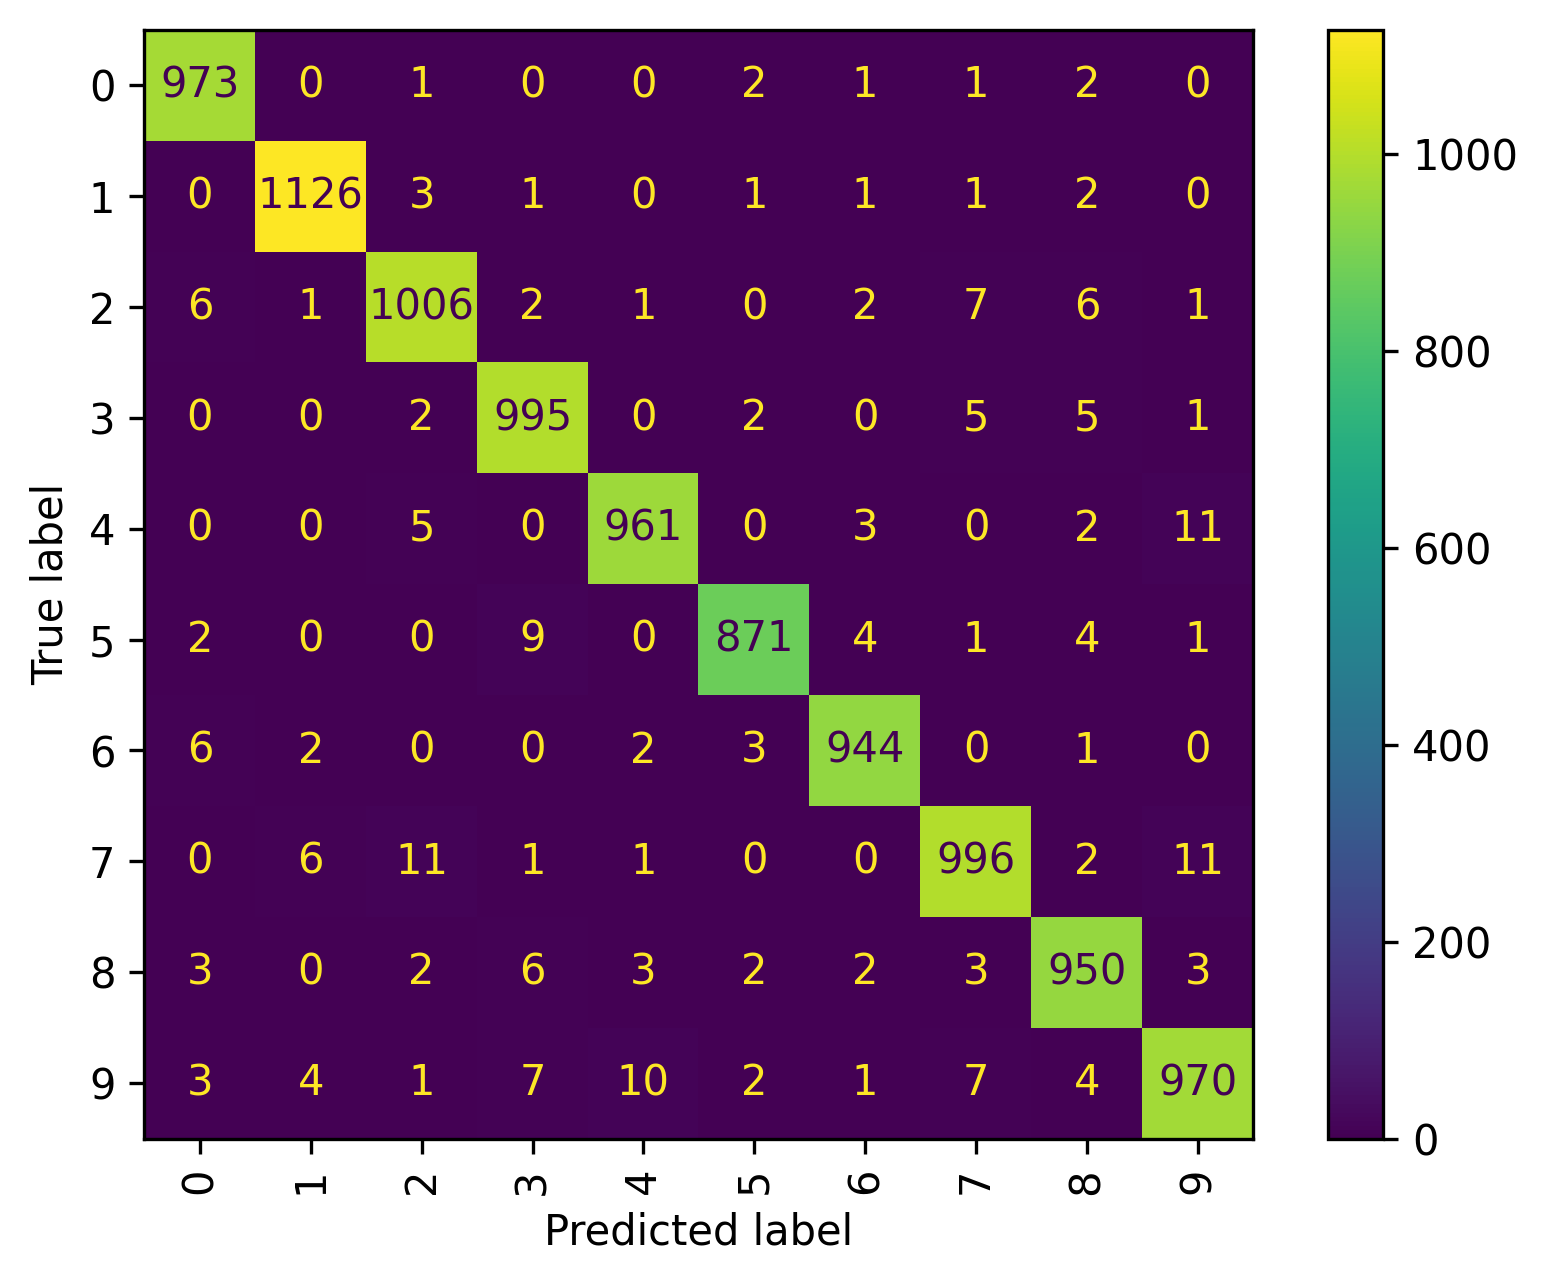
\includegraphics[width=0.6\textwidth]{confusionMatrix_SVM_MNIST.png} % Ajusta el ancho según sea necesario
    \caption{Confusion matrix for the MNIST test set using SVM}
    \label{fig:confusion-matrix}
\end{figure}

\noindent
The diagonal elements of the confusion matrix, representing the number of correctly classified samples for each digit, reveal that the model performs with high accuracy across all classes. Specifically, the model achieved the following correct classifications:

\begin{itemize}
    \item 973 instances of digit '0' were correctly identified as '0'
    \item 1126 instances of digit '1' were accurately classified.
    \item 1006 instances of digit '2' were correctly predicted, and so on.
\end{itemize}

Despite the overall high accuracy, a few misclassifications are observed. These errors are typically concentrated between visually similar digits, which is a common challenge in image classification tasks. 

\section*{6. Conclusion}
Support Vector Machines, implemented using \texttt{scikit-learn}, demonstrated strong performance on the MNIST classification task. By leveraging the RBF kernel and proper regularization, the model effectively classified high-dimensional, nonlinearly separable data. Despite its computational demands, SVM remains a powerful tool for tasks requiring high precision and robust generalization.

\section*{References}
\begin{enumerate}
    \item Cortes, C., \& Vapnik, V. (1995). Support-vector networks. \textit{Machine Learning}, 20(3), 273-297.
    \item LeCun, Y., Bottou, L., Bengio, Y., \& Haffner, P. (1998). Gradient-based learning applied to document recognition. \textit{Proceedings of the IEEE}, 86(11), 2278-2324.
    \item Pedregosa, F., Varoquaux, G., Gramfort, A., et al. (2011). Scikit-learn: Machine Learning in Python. \textit{Journal of Machine Learning Research}, 12, 2011-2825.
\end{enumerate}




\end{document}

